\documentclass[11pt]{article}
\usepackage{amsmath, amssymb, amscd, amsthm, amsfonts}
\usepackage{graphicx}
\graphicspath{ {./images/} }
\usepackage{hyperref}
\usepackage[italian]{babel}
\usepackage{tikz}
\usetikzlibrary{shapes, arrows.meta, positioning}

\oddsidemargin 0pt
\evensidemargin 0pt
\marginparwidth 40pt
\marginparsep 10pt
\topmargin -20pt
\headsep 10pt
\textheight 8.7in
\textwidth 6.65in
\linespread{1.2}

\title{Piattaforma di Gough-Stewart}
\author{Daniele Facco}
\date{}

\newtheorem{theorem}{Theorem}
\newtheorem{lemma}[theorem]{Lemma}
\newtheorem{conjecture}[theorem]{Conjecture}

\newcommand{\rr}{\mathbb{R}}

\newcommand{\al}{\alpha}
\DeclareMathOperator{\conv}{conv}
\DeclareMathOperator{\aff}{aff}

\begin{document}

\maketitle

\begin{abstract}
Studio della piattaforma di Stewart e dei suoi componenti.
\end{abstract}

\section{Servomotori}\label{servomotori}
I servomotori sono l'elemento principale nella realizzazione della piattaforma di Stewart.

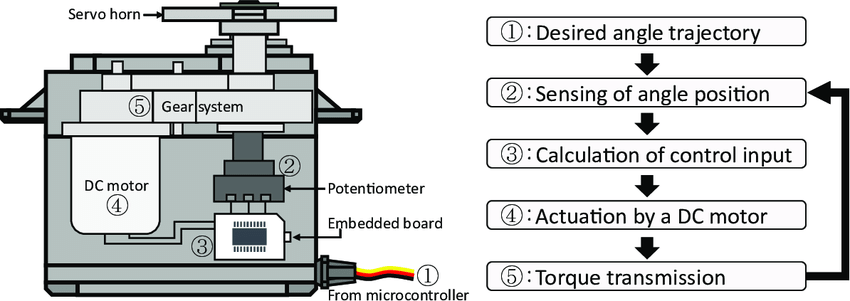
\includegraphics[scale=0.3]{Schematic-of-an-RC-servo-motor.png}

Questi motori sono controllati in modalità PWM dalla scheda Arduino tramite un'apposita libreria. Il segnale inviato ai servomotori è periodico, di periodo 20ms, e presenta uno stato on/off a livello logico per un tempo prefissato a seconda della posizione richiesta. Ad esempio la posizione 0° prevede un livello logico alto di 1ms, 90° di 1,5ms e 180° di 2ms.

Il controllo di questi elementi è gestito dalla scheda Arduino tramite uno shield che ne facilita l'installazione. Una nota particolare va fatta in merito alla potenza richiesta dai servomotori, nonostante il loro consumo in stato 'idle' sia di circa 10mW, durante il movimento questo può raggiungere oltre 300mW. É quindi necessaria una alimentazione esterna che sia in grado di fornire almeno 2A a 5V in quanto la scheda alimentata tramite usb dalla presa del computer può rivevere al massimo 1A.

\section{Piattaforma di Stewart}\label{piattaformastewart}
La piattaforma di Stewart è un particolare sistema meccanico costituito da una base su cui sono posizionati 6 attuatori di vario tipo collegati alla piattaforma superiore mediante giunti snodabili. Un esempio comune sono gli attuatori prismatici, questi sono ad esempio pistoni lineari che presentano un solo grado di libertà. Nel progetto vengono invece impiegati servomotori, questi presentano il vantaggio di essere certamente più economici rispetto agli attuatori prismatici ma il sistema risultante assume un grado di complessità superiore. Tramite opportune osservazioni matematiche è però possibile risalire ad un modello equivalente che ci garantisce un range di movimento ottimale.

\section{Robot seriali e paralleli}\label{robotserialiparalleli}
È utile enunciare la differenza tra robot di tipo seriale e parallelo per comprendere le successive implicazioni a livello matematico:

I robot seriali prevedono una serie di giunti snodabili controllati da attuatori che spesso assumono le caratteristiche di un arto antropomorfo, questi tipi di robot prendono spesso il nome di braccio meccanico e sono vastamente impiegati nell'industria meccanica.

Nei robot paralleli invece gli attuatori agiscono tutti sullo stesso elemento tramite giunti indipendenti, la piattaforma di Stewart ne è il principale esempio e le sue applicazioni sono principalmente incentrate nella realizzazione di simulatori avanzati di volo o per case automobilistiche.

Entrambi i sistemi presentano 6 gradi di libertà, indicati anche come 6DOF ma il problema matematico che li caratterizza è fondamentalmente opposto.


\section{Cinematica diretta e inversa}\label{cinematicadirettainversa}

\section{Schema logico funzionamento}\label{schema}
\begin{tikzpicture}[font=\small,thick]
 
% Start block
\node[draw,
    rounded rectangle,
    minimum width=2.5cm,
    minimum height=1cm, text width=5cm, text centered] (block1) {Caratteristiche piattaforma e servomotori};
    
    % Power and voltage variation
\node[draw,
    below=of block1,
    minimum width=3.5cm,
    minimum height=1cm
] (block2) { Calcolo $h_0$ e $\alpha_0$};
    
% Voltage and Current Measurement
\node[draw,
    trapezium, 
    trapezium left angle = 120,
    trapezium right angle = 120,
    trapezium stretches,
    below=of block2,
    minimum width=3.5cm,
    minimum height=1cm,
    text width=3cm, text centered
] (block3) { Riceve posizione $x,y,z,\varphi,\vartheta,\psi$};

\node[draw,
    below=of block3,
    minimum width=3.5cm,
    minimum height=1cm,
    text width=3cm, text centered
] (block4) {  Calcolo matrice rotazione $R_g$};

\node[draw,
    below=of block4,
    minimum width=3.5cm,
    minimum height=1cm,
    text width=2.5cm, text centered
] (block5) { Calcolo distanza $l$};

\node[draw,
    below=of block5,
    minimum width=3.5cm,
    minimum height=1cm,
    text width=3cm, text centered
] (block6) { Calcolo $\alpha$ e il corrispettivo $w$};

\node[draw,
    diamond,
    right=of block6,
    minimum width=3.5cm,
    inner sep=2, aspect=2, xshift= 1cm] (block7) {C'é collisione?};
    
\node[draw,
    right=of block7,
    minimum width=3.5cm,
    minimum height=1cm,
    text width=3.2cm, text centered, xshift=1cm
] (blocco) { Blocco sistema e accendo lampeggiate};

\node[draw,
    trapezium, 
    trapezium left angle = 120,
    trapezium right angle = 120,
    trapezium stretches,
    above=of block7,
    minimum width=3.5cm,
    minimum height=1cm,
    text width=3cm, text centered, yshift= 0.75cm
] (block8) {Imposta $w$ ai servomotori};
 
% Conditions test
\node[draw,
    diamond,
    above=of block8,
    minimum width=3.5cm,
    inner sep=2, aspect=2, yshift= 0.75cm] (block9) { Nuova posizione?};
    
\node[draw,
    above right=of block9,
    minimum width=3.5cm,
    minimum height=1cm,
    text width=3cm, text centered
] (block10) { Mantieni posizione};
 

% Arrows
\draw[-latex] (block1) edge (block2)
			  (block2) edge (block3)
			  (block3) edge (block4)
			  (block4) edge (block5)
			  (block5) edge (block6)
   			  (block6) edge (block7)
   			  (block8) edge (block9);
   
\draw[-latex] (block7) -- (blocco) node[pos=0.2,fill=white,inner sep=2]{Sì};
 
\draw[-latex] (block7) -- (block8) node[pos=0.2,fill=white,inner sep=2]{No};

\draw[-latex] (block9) -- (block3) node[pos=0.2,fill=white,inner sep=2]{Sì};
 
\draw[-latex] (block9) |- (block10) node[pos=0.2,fill=white,inner sep=2]{No};
    
\draw[-latex] (block10) |- (block9);


\end{tikzpicture}

\section{Modellizzazione problema piattaforma}\label{modello piattaforma}
\scalebox{0.6}{
\begin{tikzpicture}

\filldraw[fill=yellow!50,rotate around={-10:(0,7cm)},xshift=2cm,yshift=1cm] (0,7cm) ellipse (4cm and 2cm);
\filldraw [fill=red!50](0,0) ellipse (5cm and 2.5cm);
\draw [-latex, thick] (0,0) -- node[anchor=south]{$\hat b_i$}(5cm,0);
\draw [-latex, thick] (0,0) -- node[anchor=east]{$\hat T$}(2.15cm,7.65cm);
\draw [-latex, thick] (0,0) -- node[anchor=north]{$\hat q_i$}(6.1cm,6.95cm);
\draw [-latex, thick] (5cm,0) -- node[anchor=west]{$\hat l_i$}(6.1cm,6.95cm);
\draw[-latex, thick,rotate around={-10:(0,7cm)},xshift=2cm,yshift=1cm] (0cm,7cm) -- node[anchor=south]{$\hat p_i$}(4cm,7cm);
\filldraw [fill=black] (0,0) circle (2pt) node[yshift= -0.25cm] {$O$} node[xshift= -2cm] {Base};
\filldraw [fill=black] (5cm,0) circle (2pt) ;
\filldraw [fill=black] (2.15cm,7.65cm) circle (2pt) node[yshift= 0.25cm] {$O'$} node[xshift= -2cm] {Piattaforma};
\filldraw [fill=black] (6.1cm,6.95cm) circle (2pt);
\draw [-latex, thick] (-1,-1.5) -- node[anchor=north]{$\hat i$}(0cm,-1.5cm);
\draw [-latex, thick] (-1,-1.5) -- node[anchor=east]{$\hat k$}(-1cm,-0.5cm);
\draw [-latex, thick,rotate around={-120:(-1,-1.5cm)}] (-1,-1.5) -- node[anchor=east]{$\hat j$}(-0.5cm,-1.5cm);

\draw [-latex, thick,rotate around={-10:(0,8.5cm)}] (0,8.5) -- node[anchor=north]{$\hat {i'}$}(1cm,8.5cm);
\draw [-latex, thick,rotate around={-10:(0,8.5cm)}] (0,8.5) -- node[anchor=east]{$\hat {k'}$}(0cm,9.5cm);
\draw [-latex, thick,rotate around={-130:(0,8.5cm)}] (0,8.5) -- node[anchor=east]{$\hat {j'}$}(0.5cm,8.5cm);

\end{tikzpicture}
}
\section{Modellizzazione problema servomotori}\label{modello servo}
\scalebox{0.6}{
\begin{tikzpicture}
\filldraw [fill=black!30](0,0) rectangle (2,4);
\filldraw [fill=black] (1cm,3cm) circle (10pt);
\draw [line width=2pt] (1cm,3cm) -- node[anchor=east, xshift= 0.5cm,yshift=-0.35cm]{$m$}(4cm,2cm);
\filldraw [fill=black] (4cm,2cm) circle (3pt);
\filldraw [fill=black] (2cm,12cm) circle (3pt);
\draw [line width=2pt] (4cm,2cm) -- node[anchor=west]{$b$}(2cm,12cm);
\draw [line width=2pt,dashed] (1cm,3cm) -- node[anchor=east]{$l$}(2cm,12cm);
%\draw [<->] (3.5cm,2.2cm) arc (150:125:33.7pt);
\end{tikzpicture}
}



\bibliographystyle{alpha}
\bibliography{references} % see references.bib for bibliography management

\end{document}